\documentclass[aspectratio=169]{beamer}

\usepackage{UFtheme}


\usepackage{amsmath}
\usepackage{amssymb}
\usepackage{bm}
\usepackage{xcolor}
\usepackage{tikz}
\usetikzlibrary{positioning,arrows.meta,calc}

\definecolor{UFdarkblue}{RGB}{0,0,255}
\definecolor{UFblue}{RGB}{164,3,13}

\setbeamercolor{title}{fg=UFdarkblue}
\setbeamercolor{frametitle}{fg=UFdarkblue}
\setbeamercolor{structure}{fg=UFdarkblue}
\setbeamercolor{alerted text}{fg=UFblue}

\defbeamertemplate{footline}{titlepage footer}{
    \begin{beamercolorbox}[wd=\paperwidth,ht=2.5ex,dp=1.25ex]{page number in head/foot}
        \usebeamerfont{page number in head/foot}
        \hfill Inversion of Geophysical Data | University of Helsinki | Spring 2026 \hfill \insertframenumber\kern1em
    \end{beamercolorbox}
}
\setbeamertemplate{footline}{}

\linespread{0.94}

\setlength{\abovedisplayskip}{7pt}
\setlength{\belowdisplayskip}{7pt}
\setlength{\abovedisplayshortskip}{4pt}
\setlength{\belowdisplayshortskip}{4pt}
\addtobeamertemplate{itemize/enumerate body begin}{\setlength{\itemsep}{0.35em}}{}
\addtobeamertemplate{itemize/enumerate subbody begin}{\setlength{\itemsep}{0.2em}}{}

\setbeamercovered{invisible}

\graphicspath{{Figures/}{Lec7_2024/Figures/}}

\newcommand{\mat}[1]{{\mathbf{#1}}}
\renewcommand{\vec}[1]{\mathbf{#1}}

\newcommand{\dd}{ {\vec{d}} }
\newcommand{\dobs}{{\vec{d}^{\text{obs}}}}
\newcommand{\dpre}{{\vec{d}^{\text{pre}}}}
\newcommand{\dmean}{\left\langle \dd \right\rangle}

\newcommand{\mm}{ {\vec{m}} }
\newcommand{\delm}{ {\Delta\mm} }
\newcommand{\mest}{ {\vec{m}^{\text{est}}} }
\newcommand{\mmean}{\left\langle \mm \right\rangle}

\renewcommand{\gg}[1]{\vec{g}\left(#1\right)}
\newcommand{\ff}[1]{\vec{f}\left(#1\right)}

\newcommand{\GG}{\mat{G}}
\newcommand{\FF}{\mat{F}}
\newcommand{\II}{\mat{I}}

\newcommand{\Cd}{\mat{C}_{\dd}}
\newcommand{\Cm}{\mat{C}_{\mm,\text{prior}}}
\newcommand{\courserepo}{\texttt{https://github.com/pankajkmishra/GEOM2057}}
\newcommand{\framedfigure}[2][0.68\textheight]{%
    \includegraphics[width=\textwidth,height=#1,keepaspectratio]{#2}%
}

\title{\LARGE\textbf{Uncertainty Quantification, Bayesian Inversion \& Physics-based Machine learning}}
\author{Jochen Kamm \& \textcolor{blue}{Pankaj K Mishra}}
\date{\footnotesize\today}

\begin{document}

{
\setbeamertemplate{footline}[titlepage footer]
\begin{frame}[plain]
    \titlepage
\end{frame}
}

\begin{frame}{Learning goals}
\small

By the end of this lecture, the aim is to understand:

\begin{itemize}
    \item[--] why uncertainty quantification is central in geophysical inversion,
    \item[--] the probability essentials needed for Bayesian inversion,
    \item[--] how Bayes' rule turns the Lecture 6 misfit into a posterior distribution,
    \item[--] why direct grid or Monte Carlo integration becomes expensive,
    \item[--] what a Markov chain is and why stationarity matters,
    \item[--] how the Metropolis--Hastings algorithm samples the posterior,
    \item[--] how to read traces, marginals, predictive uncertainty, and basic MCMC diagnostics,
    \item[--] why neural networks are becoming relevant in inversion research.
\end{itemize}

\begin{alertblock}{Intuitive goal}
Move from \alert{one best model} to a \alert{probability distribution over plausible models}.
\end{alertblock}
\end{frame}

\begin{frame}{Recap and bridge from Lecture 6}
\small

In Lecture 6 we used:
\begin{itemize}
    \item[--] Newton and Gauss--Newton: local, derivative-based optimisation,
    \item[--] PSO and VFSA: derivative-free global search,
    \item[--] multiple stochastic runs: a practical way to see families of acceptable models.
\end{itemize}

\begin{alertblock}{What was missing}
An optimisation ensemble can show spread, but it is not automatically a sample from a well-defined probability distribution.
\end{alertblock}

\begin{itemize}
    \item[--] Bayesian inversion defines the target distribution: $p(\mm\mid\dobs)$.
    \item[--] MCMC gives us a practical way to sample that distribution when direct calculation is too expensive.
\end{itemize}
\end{frame}

\begin{frame}{Why uncertainty matters in geophysics}
\small

\textbf{A geophysical answer is rarely just one model.} Decisions depend on the spread of plausible models.

\begin{columns}[T]
\column{0.5\textwidth}
\begin{block}{Examples}
\begin{itemize}
    \item[--] How deep is the reservoir?
    \item[--] How thick is the conductive layer?
    \item[--] Is an anomaly shallow and small, or deep and large?
    \item[--] Which features are required by the data?
\end{itemize}
\end{block}

\column{0.5\textwidth}
\begin{block}{Sources of uncertainty}
\begin{itemize}
    \item[--] noisy data,
    \item[--] sparse or uneven coverage,
    \item[--] non-unique forward responses,
    \item[--] imperfect physics and parameterization.
\end{itemize}
\end{block}
\end{columns}

\begin{alertblock}{Bayesian question}
Which Earth models are plausible, and how plausible is each one, given the data and assumptions?
\end{alertblock}
\end{frame}

\begin{frame}{What Is a Posterior?}
\small

In Bayesian inversion, a \alert{posterior} is our updated state of knowledge \alert{after seeing the data}.

\begin{block}{Plain-language idea}
\begin{itemize}
    \item[--] Before seeing the data, we have prior beliefs about plausible models.
    \item[--] The data then favor some models and rule out others.
    \item[--] The posterior tells us which models remain plausible after combining both pieces of information.
\end{itemize}
\end{block}

\begin{alertblock}{Informal reading}
Posterior = \alert{what we believe now}, after using the observations.
\end{alertblock}
\end{frame}

\begin{frame}{Three levels of answer}
\small

\begin{block}{What is the model?}
\begin{itemize}
    \item[--] \alert{Level 1 -- one model}: $\mest$ from a deterministic inversion.
    \item[--] \alert{Level 2 -- an ensemble}: several acceptable models from repeated stochastic searches.
    \item[--] \alert{Level 3 -- a posterior}: a probability distribution $p(\mm\mid\dobs)$ over models.
\end{itemize}
\end{block}

\begin{alertblock}{Interpretation}
The posterior is stronger than a collection of good models because it attaches probability to model space.
\end{alertblock}

\begin{itemize}
    \item[--] Marginals tell us uncertainty in individual parameters.
    \item[--] Joint distributions reveal trade-offs and correlations.
    \item[--] Posterior predictions show the range of data responses still consistent with the observations.
\end{itemize}
\end{frame}

\section{Probability Essentials}

\begin{frame}{Start with a simple measurement: height}
\small

Suppose we travel across Finland and record the heights of many people:
\[
171\text{ cm},\ 182\text{ cm},\ 176\text{ cm},\ 168\text{ cm},\ 174\text{ cm},\ \dots
\]

\begin{itemize}
    \item[--] With only a few measurements, the values feel random.
    \item[--] After many measurements, a pattern appears.
    \item[--] Most people cluster near a middle value.
    \item[--] Very short and very tall heights are less common.
\end{itemize}

\begin{alertblock}{Key intuition}
Uncertainty does not mean \alert{no structure}. It means we do not know the exact value, but values occur with different frequencies.
\end{alertblock}
\end{frame}

\begin{frame}{From repeated measurements to a PDF}
\small

If we sort many heights into bins, we get counts.

\begin{columns}[T]
\column{0.48\textwidth}
\begin{block}{Example counts}
\begin{tabular}{ll}
165--170 cm & 1800 \\
170--175 cm & 2600 \\
175--180 cm & 2300 \\
180--185 cm & 1300
\end{tabular}
\end{block}

\column{0.48\textwidth}
\begin{block}{Interpretation}
\begin{itemize}
    \item[--] Divide by the total number of people.
    \item[--] Counts become fractions.
    \item[--] Fractions approximate probabilities.
\end{itemize}
\end{block}
\end{columns}

\begin{alertblock}{Continuous-variable shift}
For height, the probability of one exact value is zero. Probability lives on intervals:
\[
P(170 \leq H \leq 175).
\]
\end{alertblock}
\end{frame}

\begin{frame}{What a probability density function means}
\small

A random variable assigns numerical values to uncertain outcomes. For a continuous variable, we use a probability density function (PDF).

\begin{block}{Continuous PDF}
\[
p_H(h) \geq 0,
\qquad
\int_{-\infty}^{\infty} p_H(h)\,dh = 1.
\]
\end{block}

\begin{alertblock}{Most important idea}
The height of the curve is \alert{not} probability. Probability is \alert{area under the curve}:
\[
P(a\leq H\leq b)=\int_a^b p_H(h)\,dh.
\]
\end{alertblock}

\begin{itemize}
    \item[--] High density means nearby values are common.
    \item[--] Low density means nearby values are rare.
    \item[--] Total area must be one because all possibilities must be somewhere.
\end{itemize}
\end{frame}

\begin{frame}{Why a bell curve appears so often}
\small

Human height is affected by many small contributions:

\begin{itemize}
    \item[--] genetics,
    \item[--] nutrition,
    \item[--] childhood health,
    \item[--] random biological variation.
\end{itemize}

When many small effects combine, a bell-shaped distribution often appears. This is the Gaussian or normal distribution:
\[
p(x\mid\mu,\sigma)
=
\frac{1}{\sigma\sqrt{2\pi}}
\exp\left[
-\frac{(x-\mu)^2}{2\sigma^2}
\right].
\]

\begin{block}{Meaning of the parameters}
\begin{itemize}
    \item[--] $\mu$: center or mean.
    \item[--] $\sigma$: spread or standard deviation.
\end{itemize}
\end{block}
\end{frame}

\begin{frame}{What Height Data Look Like}
\small

\begin{center}
\framedfigure{L7_01_height_pdf_intuition.png}
\end{center}

\vspace{-0.15cm}
\begin{block}{Demo file}
\texttt{L7/01-height-pdf-intuition.jl} shows how a histogram, a smooth PDF, and interval probability connect.
\end{block}
\end{frame}

\begin{frame}{Now add a second measurement: weight}
\small

Suppose each person gives us a pair of numbers:
\[
(\text{height},\text{weight}).
\]

\begin{itemize}
    \item[--] We no longer ask how common one value is.
    \item[--] We ask how common \alert{combinations} are.
    \item[--] Some combinations are plausible: tall and heavy, short and light.
    \item[--] Some combinations are less common: very tall and very light.
\end{itemize}

\begin{alertblock}{New object}
For two variables, probability is described by a \alert{joint PDF} $p(h,w)$.
\end{alertblock}
\end{frame}

\begin{frame}{Joint PDFs, marginals, and conditionals}
\small

The joint PDF tells us where combinations of height and weight are concentrated.

\begin{block}{Marginalization}
If we stop caring about weight and only want height, we sum over all possible weights:
\[
p(h)=\int p(h,w)\,dw.
\]
Likewise,
\[
p(w)=\int p(h,w)\,dh.
\]
\end{block}

\begin{block}{Conditional probability}
If height is already known, the probability of weight becomes
\[
p(w\mid h)=\frac{p(h,w)}{p(h)},
\qquad p(h)>0.
\]
\end{block}
\end{frame}

\begin{frame}{Dependence, correlation, and trade-offs}
\small

Height and weight are usually related, so the joint PDF is often tilted rather than circular.

\begin{itemize}
    \item[--] If two variables are independent, then $p(h,w)=p(h)p(w)$.
    \item[--] If they are dependent, knowing one changes what values of the other remain plausible.
    \item[--] In inverse problems, this becomes a parameter trade-off.
\end{itemize}

\begin{alertblock}{Why this matters later}
Posterior trade-offs in geophysics are the same idea: one parameter can increase while another decreases, and the data still fit.
\end{alertblock}
\end{frame}

\begin{frame}{How Height and Weight Vary Together}
\small

\begin{center}
\framedfigure{L7_02_height_weight_joint_pdf.png}
\end{center}

\vspace{-0.15cm}
\begin{block}{Demo file}
\texttt{L7/02-height-weight-joint-pdf.jl} shows samples, the joint density, and how correlation tilts the high-probability region.
\end{block}
\end{frame}

\begin{frame}{From People to Earth Models}
\small

In geophysics, the uncertain quantities are not height and weight. They are model parameters such as

\begin{itemize}
    \item[--] velocity,
    \item[--] density,
    \item[--] conductivity,
    \item[--] layer thickness.
\end{itemize}

\begin{block}{Same probability ideas, different variables}
\begin{itemize}
    \item[--] one parameter $\rightarrow$ one marginal PDF,
    \item[--] two parameters $\rightarrow$ one joint PDF,
    \item[--] many parameters $\rightarrow$ a high-dimensional probability distribution.
\end{itemize}
\end{block}

\begin{alertblock}{Bridge to Bayes}
The goal of Bayesian inversion is to describe which Earth models are plausible after we have observed the data.
\end{alertblock}
\end{frame}

\section{Bayesian Inversion}

\begin{frame}{Bayes' rule}
\small

\begin{alertblock}{General form}
\[
p(\vec{x}\mid\vec{y})
=
\frac{p(\vec{y}\mid\vec{x})p(\vec{x})}{p(\vec{y})}.
\]
\end{alertblock}

\begin{block}{Inverse-problem form}
\[
p(\mm\mid\dobs)
=
\frac{p(\dobs\mid\mm)p(\mm)}{p(\dobs)}.
\]
\end{block}

\begin{itemize}
    \item[--] $p(\mm\mid\dobs)$: posterior distribution over models.
    \item[--] $p(\dobs\mid\mm)$: likelihood, how well model $\mm$ predicts the data.
    \item[--] $p(\mm)$: prior information before observing the data.
    \item[--] $p(\dobs)$: evidence or normalizing constant.
\end{itemize}
\end{frame}

\begin{frame}{The evidence}
\small

The evidence is obtained by integrating over all possible models:
\[
p(\dobs)
=
\int p(\dobs\mid\mm)p(\mm)\,d\mm.
\]

\begin{alertblock}{Why this term matters}
It normalizes the posterior so that
\[
\int p(\mm\mid\dobs)\,d\mm = 1.
\]
\end{alertblock}

\begin{itemize}
    \item[--] For parameter estimation, we often use the unnormalized posterior
    \[
    p(\mm\mid\dobs)\propto p(\dobs\mid\mm)p(\mm).
    \]
    \item[--] For model comparison, the evidence itself can matter.
    \item[--] In high dimensions, the evidence integral is usually the hard part.
\end{itemize}
\end{frame}

\begin{frame}{Gaussian likelihood for geophysical data}
\small

Assume
\[
\dobs = \gg{\mm}+\boldsymbol\varepsilon,
\qquad
\boldsymbol\varepsilon\sim\mathcal{N}(\vec{0},\Cd).
\]

Then
\[
p(\dobs\mid\mm)
=
\frac{1}{(2\pi)^{N/2}|\Cd|^{1/2}}
\exp\left[
-\frac{1}{2}
\left(\dobs-\gg{\mm}\right)^T\Cd^{-1}
\left(\dobs-\gg{\mm}\right)
\right].
\]

\begin{alertblock}{Lecture 6 connection}
\[
\chi_d^2(\mm)
=
\left(\dobs-\gg{\mm}\right)^T\Cd^{-1}
\left(\dobs-\gg{\mm}\right),
\qquad
\log p(\dobs\mid\mm)=\text{const}-\frac{1}{2}\chi_d^2(\mm).
\]
\end{alertblock}
\end{frame}

\begin{frame}{Priors in inverse problems}
\small

A prior describes model information before the current data are used.

\begin{columns}[T]
\column{0.5\textwidth}
\begin{block}{Bounded uniform prior}
\[
p(\mm)=
\begin{cases}
\text{constant}, & \mm\in\mathcal{M},\\
0, & \mm\notin\mathcal{M}.
\end{cases}
\]
\end{block}
Useful when the main prior information is a physically plausible range.

\column{0.5\textwidth}
\begin{block}{Gaussian prior}
\[
p(\mm)
\propto
\exp\left[
-\frac{1}{2}
(\mm-\mmean)^T\Cm^{-1}(\mm-\mmean)
\right].
\]
\end{block}
Useful when a reference model and covariance are meaningful.
\end{columns}
\end{frame}

\begin{frame}{MAP estimate and the Lecture 6 objective}
\small

The maximum a posteriori model is
\[
\mm_{\mathrm{MAP}}
=
\arg\max_{\mm}p(\mm\mid\dobs)
=
\arg\min_{\mm}\left[-\log p(\dobs\mid\mm)-\log p(\mm)\right].
\]

With Gaussian data errors and a Gaussian prior,
\[
-\log p(\mm\mid\dobs)
=
\frac{1}{2}
\left(\dobs-\gg{\mm}\right)^T\Cd^{-1}
\left(\dobs-\gg{\mm}\right)
+
\frac{1}{2}
(\mm-\mmean)^T\Cm^{-1}(\mm-\mmean)
+\text{const}.
\]

\begin{alertblock}{Key bridge}
The regularized least-squares objective from Lecture 6 is the negative log-posterior under Gaussian assumptions.
\end{alertblock}
\end{frame}

\begin{frame}{How can we compute the posterior?}
\small

\begin{block}{Monte Carlo idea}
Draw many model samples from the prior:
\[
\mm_i\sim p(\mm),
\qquad i=1,\dots,N.
\]

Each sample $\mm_i$ is one possible Earth model before seeing the data.
\end{block}

\begin{itemize}
    \item[--] Then evaluate how well each sample explains the data through the likelihood $p(\dobs\mid\mm_i)$.
    \item[--] Samples that fit the data well should matter more.
    \item[--] Samples that fit badly should matter less.
\end{itemize}
\end{frame}

\begin{frame}{How do the weights work?}
\small

Because the models were drawn from the prior, the data only need to reweight them:
\[
w_i\propto p(\dobs\mid\mm_i),
\qquad \sum_i w_i=1.
\]

\begin{alertblock}{Meaning of $w_i$}
$w_i$ tells us how much posterior probability is assigned to sample $\mm_i$.
\end{alertblock}

\begin{itemize}
    \item[--] Large $w_i$: this model stays plausible after seeing the data.
    \item[--] Small $w_i$: this model is strongly disfavored by the data.
    \item[--] The weighted sample cloud is a discrete approximation of the posterior.
\end{itemize}
\end{frame}

\begin{frame}{How do we get model parameters from the weights?}
\small

Once we have samples $\mm_i$ and weights $w_i$, we can estimate model quantities.

\begin{block}{Posterior mean model}
\[
\mmean_{\mathrm{post}}
\approx
\sum_{i=1}^{N} w_i\,\mm_i.
\]
\end{block}

For one parameter, for example $m_k$,
\[
\langle m_k\rangle
\approx
\sum_{i=1}^{N} w_i\,m_{i,k}.
\]

\begin{itemize}
    \item[--] This gives an average model, weighted by posterior plausibility.
    \item[--] We can also compute credible intervals and marginal PDFs from the same weighted samples.
    \item[--] If we want one best sample, we can take the sample with the largest weight.
    \item[--] For predicted data, use the same idea: $\sum_i w_i\,\gg{\mm_i}$.
    \item[--] So the goal is not only one model, but a weighted family of plausible models.
\end{itemize}
\end{frame}

\begin{frame}{Why MCMC?}
\small

Direct methods waste many evaluations in regions with tiny posterior probability.

\begin{alertblock}{MCMC idea}
Construct a dependent sequence of models
\[
\mm^{(1)},\mm^{(2)},\dots,\mm^{(N)}
\]
whose long-run distribution is the target posterior $p(\mm\mid\dobs)$.
\end{alertblock}

\begin{itemize}
    \item[--] The samples are correlated, not independent.
    \item[--] But if the chain is built correctly and run long enough, the sample cloud represents the posterior.
    \item[--] We can then estimate marginal PDFs, means, credible intervals, correlations, and predictive uncertainty.
\end{itemize}
\end{frame}

\section{Markov Chains}

\begin{frame}{What is a Markov chain?}
\small

A Markov chain is a random process where the next step depends only on \alert{where we are now}, not on the full history.

\begin{block}{Finite-state example}
For states Sunny, Cloudy, Rainy, the transition matrix can be
\[
P=
\begin{bmatrix}
0.7 & 0.2 & 0.1\\
0.3 & 0.4 & 0.3\\
0.2 & 0.3 & 0.5
\end{bmatrix}.
\]
\end{block}

\begin{itemize}
    \item[--] Each row tells us what tomorrow's weather could be, given today's weather.
    \item[--] For example, if today is Sunny, the first row says tomorrow is most likely Sunny again, but Cloudy or Rainy are also possible.
    \item[--] The important idea is memory of just one step: today influences tomorrow.
\end{itemize}
\end{frame}

\begin{frame}{Stationary distribution: weather-chain example}
\small

\begin{block}{Stationary distribution}
A stationary distribution is the long-run balance of time spent in each state.
\end{block}

\begin{alertblock}{Why this matters for MCMC}
In MCMC we design the transition rule so that the posterior is the stationary distribution.
\end{alertblock}

\begin{itemize}
    \item[--] Imagine running the weather model for a very long time.
    \item[--] At first, the proportions depend on the starting day.
    \item[--] After many steps, those proportions settle to stable values.
    \item[--] Those stable values are the stationary distribution.
    \item[--] In the weather example, the animation shows these running frequencies settling down.
\end{itemize}
\end{frame}

\begin{frame}{A Simple Weather Chain}
\small

\begin{center}
\framedfigure[0.70\textheight]{L7_04_markov_chain.png}
\end{center}

\vspace{-0.15cm}
\begin{block}{Demo file}
\texttt{L7/04-markov-chain-demo.jl} simulates the Sunny--Cloudy--Rainy chain, saves a simpler figure, and writes a GIF showing frequencies converging toward the stationary distribution.
\end{block}
\end{frame}

\section{Metropolis--Hastings}

\begin{frame}{MCMC target distribution}
\small

For Bayesian inversion, the target density is the posterior:
\[
\pi(\mm) = p(\mm\mid\dobs)
\propto
p(\dobs\mid\mm)p(\mm).
\]

\begin{alertblock}{Important practical point}
Metropolis--Hastings only needs the posterior up to a proportionality constant. The evidence $p(\dobs)$ cancels in the acceptance ratio.
\end{alertblock}

\begin{itemize}
    \item[--] We need to evaluate $\log p(\dobs\mid\mm)+\log p(\mm)$.
    \item[--] We do not need to compute the full evidence integral.
    \item[--] This is one reason MCMC is so useful for inverse problems.
\end{itemize}
\end{frame}

\begin{frame}{Metropolis--Hastings algorithm}
\footnotesize

Both methods follow the same outer loop: current model $\rightarrow$ proposal $\rightarrow$ accept or reject.

\begin{columns}[T]
\column{0.48\textwidth}
\begin{block}{VFSA reminder}
Goal: find a low-misfit model.

\[
P_{\mathrm{acc}} =
\begin{cases}
1, & \Delta\Phi \leq 0,\\
\exp\!\left(-\dfrac{\Delta\Phi}{T}\right), & \Delta\Phi > 0.
\end{cases}
\]
\end{block}

\column{0.48\textwidth}
\begin{block}{Metropolis--Hastings}
Goal: sample the posterior.

Proposal: $\mm'\sim q(\mm'\mid\mm_i)$.

\[
\alpha
=
\min\left[
1,
\frac{\pi(\mm')q(\mm_i\mid\mm')}
{\pi(\mm_i)q(\mm'\mid\mm_i)}
\right].
\]
\end{block}
\end{columns}

\begin{itemize}
    \item[--] Draw $u\sim U(0,1)$ and accept if $u\leq\alpha$.
    \item[--] If rejected, repeat the current model.
    \item[--] Main difference: VFSA is an optimizer; MH is a sampler.
\end{itemize}
\end{frame}

\begin{frame}{Use log probabilities}
\small

In practice we compute with log probabilities to avoid numerical underflow.

\begin{block}{General log acceptance}
\[
\log\alpha
=
\min\left[
0,\,
\log\pi(\mm')-\log\pi(\mm_i)
+
\log q(\mm_i\mid\mm')
-
\log q(\mm'\mid\mm_i)
\right].
\]
\end{block}

\begin{alertblock}{Acceptance test}
Draw $u\sim U(0,1)$ and accept if
\[
\log u < \log\alpha.
\]
\end{alertblock}
\end{frame}

\begin{frame}{The Posterior Used in This Example}
\small

The demo uses the Lecture 6 hard forward model:
\[
d_i^{\mathrm{pre}}
=
m_1\exp\left[-\left(\frac{t_i}{m_2}\right)^2\right]+m_3.
\]

The prior is bounded uniform:
\[
\mm\in[m^{\min}_1,m^{\max}_1]\times[m^{\min}_2,m^{\max}_2]\times[m^{\min}_3,m^{\max}_3].
\]

\begin{alertblock}{Log posterior}
\[
\log\pi(\mm)
=
\begin{cases}
-\dfrac{1}{2\sigma_d^2}
\left\|\dobs-\gg{\mm}\right\|_2^2 + \text{const},
& \mm\ \text{inside bounds},\\[0.25cm]
-\infty,
& \mm\ \text{outside bounds}.
\end{cases}
\]
\end{alertblock}
\end{frame}

\begin{frame}{Full MCMC inversion algorithm}
\footnotesize

Given observed data $\dobs$, a prior $p(\mm)$, a likelihood $p(\dobs\mid\mm)$, and a starting model $\mm_0$:

\begin{enumerate}
    \item[--] Choose the number of samples, burn-in length, and a proposal rule $q(\mm'\mid\mm_i)$.
    \item[--] Start from the current model $\mm_i$ and evaluate its log posterior
    \[
    \log\pi(\mm_i)=\log p(\dobs\mid\mm_i)+\log p(\mm_i).
    \]
    \item[--] Propose a trial model $\mm'\sim q(\mm'\mid\mm_i)$.
    \item[--] Evaluate the trial log posterior $\log\pi(\mm')$.
    \item[--] Compute the log acceptance probability
    \[
    \log\alpha=
    \min\left[0,\,\log\pi(\mm')-\log\pi(\mm_i)+\log q(\mm_i\mid\mm')-\log q(\mm'\mid\mm_i)\right].
    \]
    \item[--] Draw $u\sim U(0,1)$. If $\log u<\log\alpha$, accept the proposal; otherwise keep the current model.
    \item[--] Store the resulting sample and repeat until the chain is long enough.
    \item[--] Discard burn-in, then use the remaining samples to compute marginals, means, intervals, and predictive uncertainty.
\end{enumerate}

\begin{alertblock}{Output}
The result is not one best model, but a sample-based approximation of the posterior distribution over plausible models.
\end{alertblock}
\end{frame}

\begin{frame}{Sampling the Posterior}
\small

The MCMC demo and all lecture code are in the repository
\[
\courserepo
\]

\begin{block}{Main files}
\begin{itemize}
    \item[--] \texttt{L6/05-problem-setup-hard.jl}: hard forward model and objective helpers.
    \item[--] \texttt{L6/06-data-generation-hard.jl}: repeatable sparse/noisy synthetic data.
    \item[--] \texttt{L7/05-metropolis-hastings-geophysical.jl}: posterior sampling and CairoMakie plots.
\end{itemize}
\end{block}

\begin{alertblock}{Output}
The output shows trace behavior, parameter uncertainty, and predictive uncertainty.
\end{alertblock}
\end{frame}

\begin{frame}{One MCMC Result}
\small

\begin{center}
\framedfigure[0.78\textheight]{L7_05_metropolis_hastings_geophysical.png}
\end{center}
\end{frame}

\begin{frame}{How to read an MCMC result}
\small

\begin{block}{Trace plots}
\begin{itemize}
    \item[--] Check whether the chain has moved away from its starting point.
    \item[--] Look for poor mixing, long drifts, or chains stuck in one region.
\end{itemize}
\end{block}

\begin{block}{Marginal histograms}
\begin{itemize}
    \item[--] Summarize uncertainty in one parameter at a time.
    \item[--] Report posterior median, mean, and credible intervals.
\end{itemize}
\end{block}

\begin{block}{Predictive uncertainty}
\begin{itemize}
    \item[--] Push posterior samples through the forward model.
    \item[--] The predictive band shows which data responses remain plausible.
\end{itemize}
\end{block}
\end{frame}

\begin{frame}{Burn-in, correlation, and effective samples}
\small

MCMC samples are not independent draws.

\begin{itemize}
    \item[--] \alert{Burn-in}: early samples may reflect the starting model more than the posterior.
    \item[--] \alert{Autocorrelation}: nearby samples in the chain are usually similar.
    \item[--] \alert{Effective sample size}: the number of independent samples that would contain similar information.
    \item[--] \alert{Multiple chains}: starting from different regions helps reveal non-convergence.
\end{itemize}

\begin{alertblock}{Practical warning}
A long chain is not automatically a good chain. We still need diagnostics and geological judgment.
\end{alertblock}
\end{frame}

\begin{frame}{What MCMC gives and what it does not}
\small

\begin{columns}[T]
\column{0.5\textwidth}
\begin{block}{MCMC gives}
\begin{itemize}
    \item[--] posterior samples,
    \item[--] parameter uncertainty,
    \item[--] parameter trade-offs,
    \item[--] posterior predictive checks.
\end{itemize}
\end{block}

\column{0.5\textwidth}
\begin{block}{MCMC does not automatically give}
\begin{itemize}
    \item[--] a perfect answer from a short run,
    \item[--] independence between samples,
    \item[--] protection from a wrong likelihood,
    \item[--] protection from a bad prior or bad forward model.
\end{itemize}
\end{block}
\end{columns}

\begin{alertblock}{Main message}
Bayesian inversion quantifies uncertainty conditional on the assumptions. If the assumptions change, the posterior can change too.
\end{alertblock}
\end{frame}

\begin{frame}{Common MCMC extensions}
\small

Metropolis--Hastings is the simplest useful entry point. Many extensions keep the same goal but improve efficiency or robustness.

\begin{block}{Examples}
\begin{itemize}
    \item[--] \textbf{Gibbs sampling}: sample from conditional distributions when they are available.
    \item[--] \textbf{Adaptive Metropolis}: adjust proposal covariance during warm-up.
    \item[--] \textbf{Parallel tempering}: run chains at different temperatures to explore multi-modal targets.
    \item[--] \textbf{Sequential Monte Carlo}: move a population of weighted particles through a sequence of distributions.
    \item[--] \textbf{Ensemble samplers}: use an ensemble of walkers to adapt proposal directions.
\end{itemize}
\end{block}

\begin{alertblock}{Core idea}
Build a chain whose stationary distribution is the posterior.
\end{alertblock}
\end{frame}

\section{Implicit Neural Representations}

\begin{frame}{Why inversion looks like training}
\small

\begin{columns}[T]
\column{0.5\textwidth}
\begin{block}{Geophysical inversion}
\begin{itemize}
    \item[--] Start with unknown model parameters.
    \item[--] Predict data with a forward model.
    \item[--] Compare predicted and observed data.
    \item[--] Update parameters to reduce the mismatch.
\end{itemize}
\end{block}

\column{0.5\textwidth}
\begin{block}{Neural-network training}
\begin{itemize}
    \item[--] Start with unknown weights.
    \item[--] Predict outputs with the network.
    \item[--] Compare predicted and target outputs.
    \item[--] Update weights to reduce the loss.
\end{itemize}
\end{block}
\end{columns}

\begin{alertblock}{Big similarity}
Both problems search for parameters by repeatedly predicting, comparing, and updating.
\end{alertblock}
\end{frame}

\begin{frame}{Can neural networks help inversion?}
\footnotesize

Yes. There are many ways to use neural networks in inversion, and this is now a very active research area.

\begin{block}{One direction we are exploring}
\textbf{Physics-informed machine learning via implicit neural representation (INR).}

Instead of storing one value in each cell, we train a neural network that maps coordinates to Earth properties.
\end{block}

\begin{center}
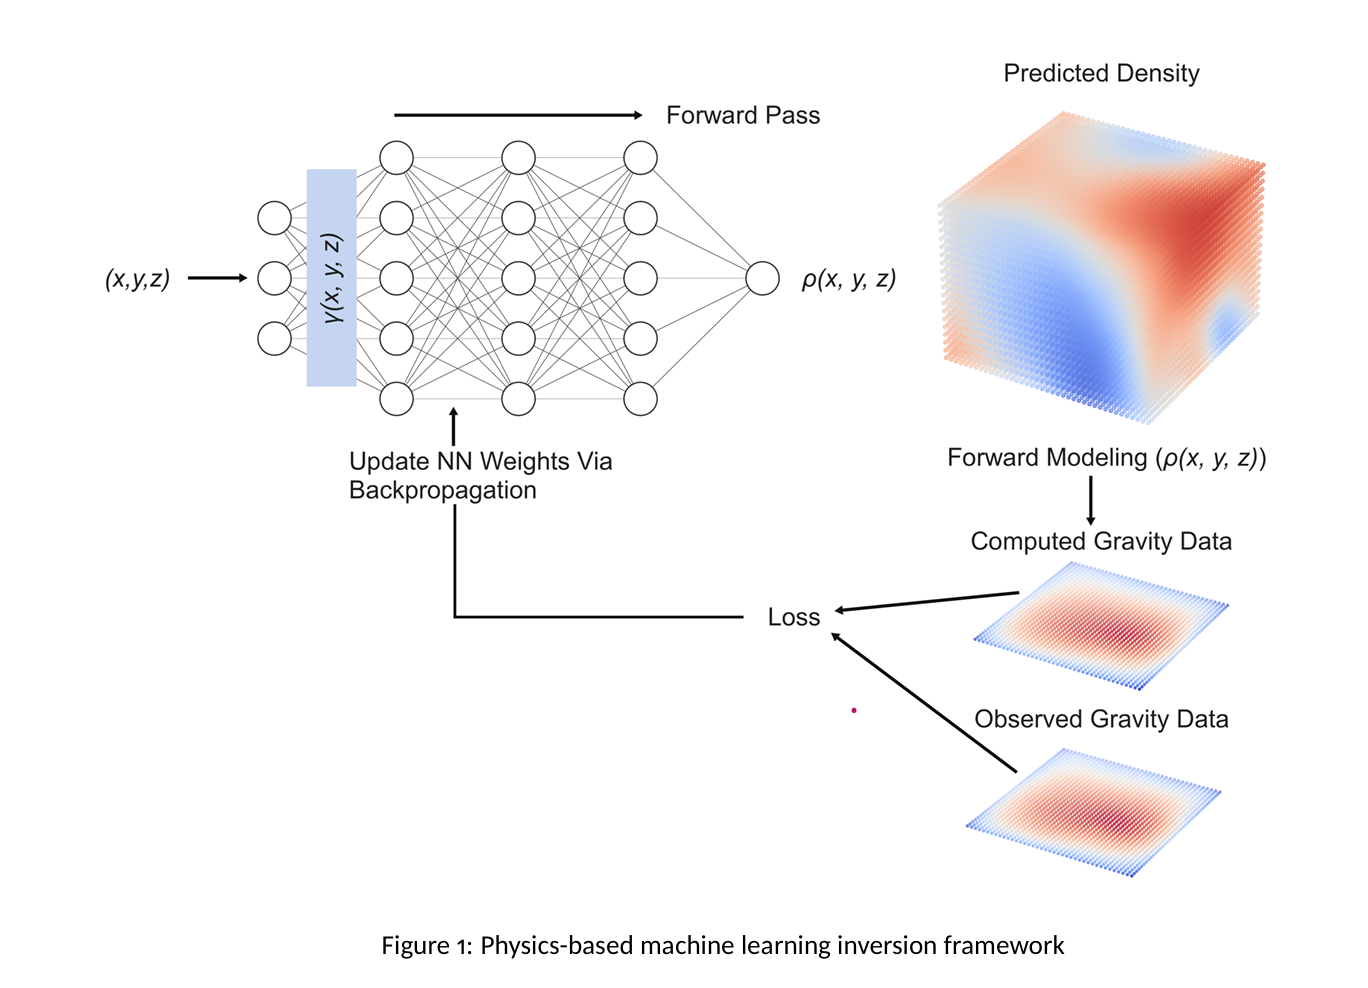
\includegraphics[width=0.78\textwidth,height=0.38\textheight,keepaspectratio]{INR.png}
\end{center}

\begin{alertblock}{Read more}
Please read \textit{Three-dimensional inversion of gravity data using implicit neural representations and scientific machine learning} (arXiv:2510.17876). The paper includes Python codes.
\end{alertblock}
\end{frame}

\section{Conclusions}

\begin{frame}{So what did we learn?}
\footnotesize

\begin{itemize}
    \item[--] Uncertainty matters because many Earth models can explain noisy, incomplete data.
    \item[--] Bayes' rule combines likelihood and prior information into a posterior distribution.
    \item[--] With Gaussian data errors, the Lecture 6 least-squares misfit is the negative log-likelihood up to a constant.
    \item[--] With a Gaussian prior, regularization becomes a prior penalty in the negative log-posterior.
    \item[--] Grid search and plain Monte Carlo are transparent but scale poorly with dimension.
    \item[--] A Markov chain has a long-run stationary distribution.
    \item[--] Metropolis--Hastings constructs a chain whose stationary distribution is the posterior.
    \item[--] MCMC output should be read through traces, marginals, and diagnostics.
    \item[--] Geophysical inversion and neural-network training share the same predict-compare-update structure.
    \item[--] Neural networks can be used for inversion in many ways, and this is a popular research direction.
    \item[--] One example is physics-informed machine learning with implicit neural representations.
\end{itemize}

\begin{alertblock}{Take-home message}
Bayesian inversion helps us describe plausible Earth models, and modern machine-learning ideas may give us new ways to represent and solve these problems.
\end{alertblock}
\end{frame}

\end{document}
